\section{More Attention Heads in Dormant and Active Phase}\label{sec:more_heads}
We demonstrate a head with clear \textit{active-dormant mechanism} in Figure~\ref{fig:dormant_heads_domain_dependent}. 
In this section, we present two more active-dormant heads in Llama 2-7B-Base, in \Cref{fig:llama_l16h20,fig:llama_l16h28}, which are more difficult to interpret than Layer 16 Head 25, but become dormant on some inputs and remain active on others. 
% \sm{Explain in more details. Now the figure is far away from the text. }

\begin{figure}[h]
    \centering
    \begin{subfigure}{0.575\textwidth}
        \centering 
        \caption{Attention patterns}
        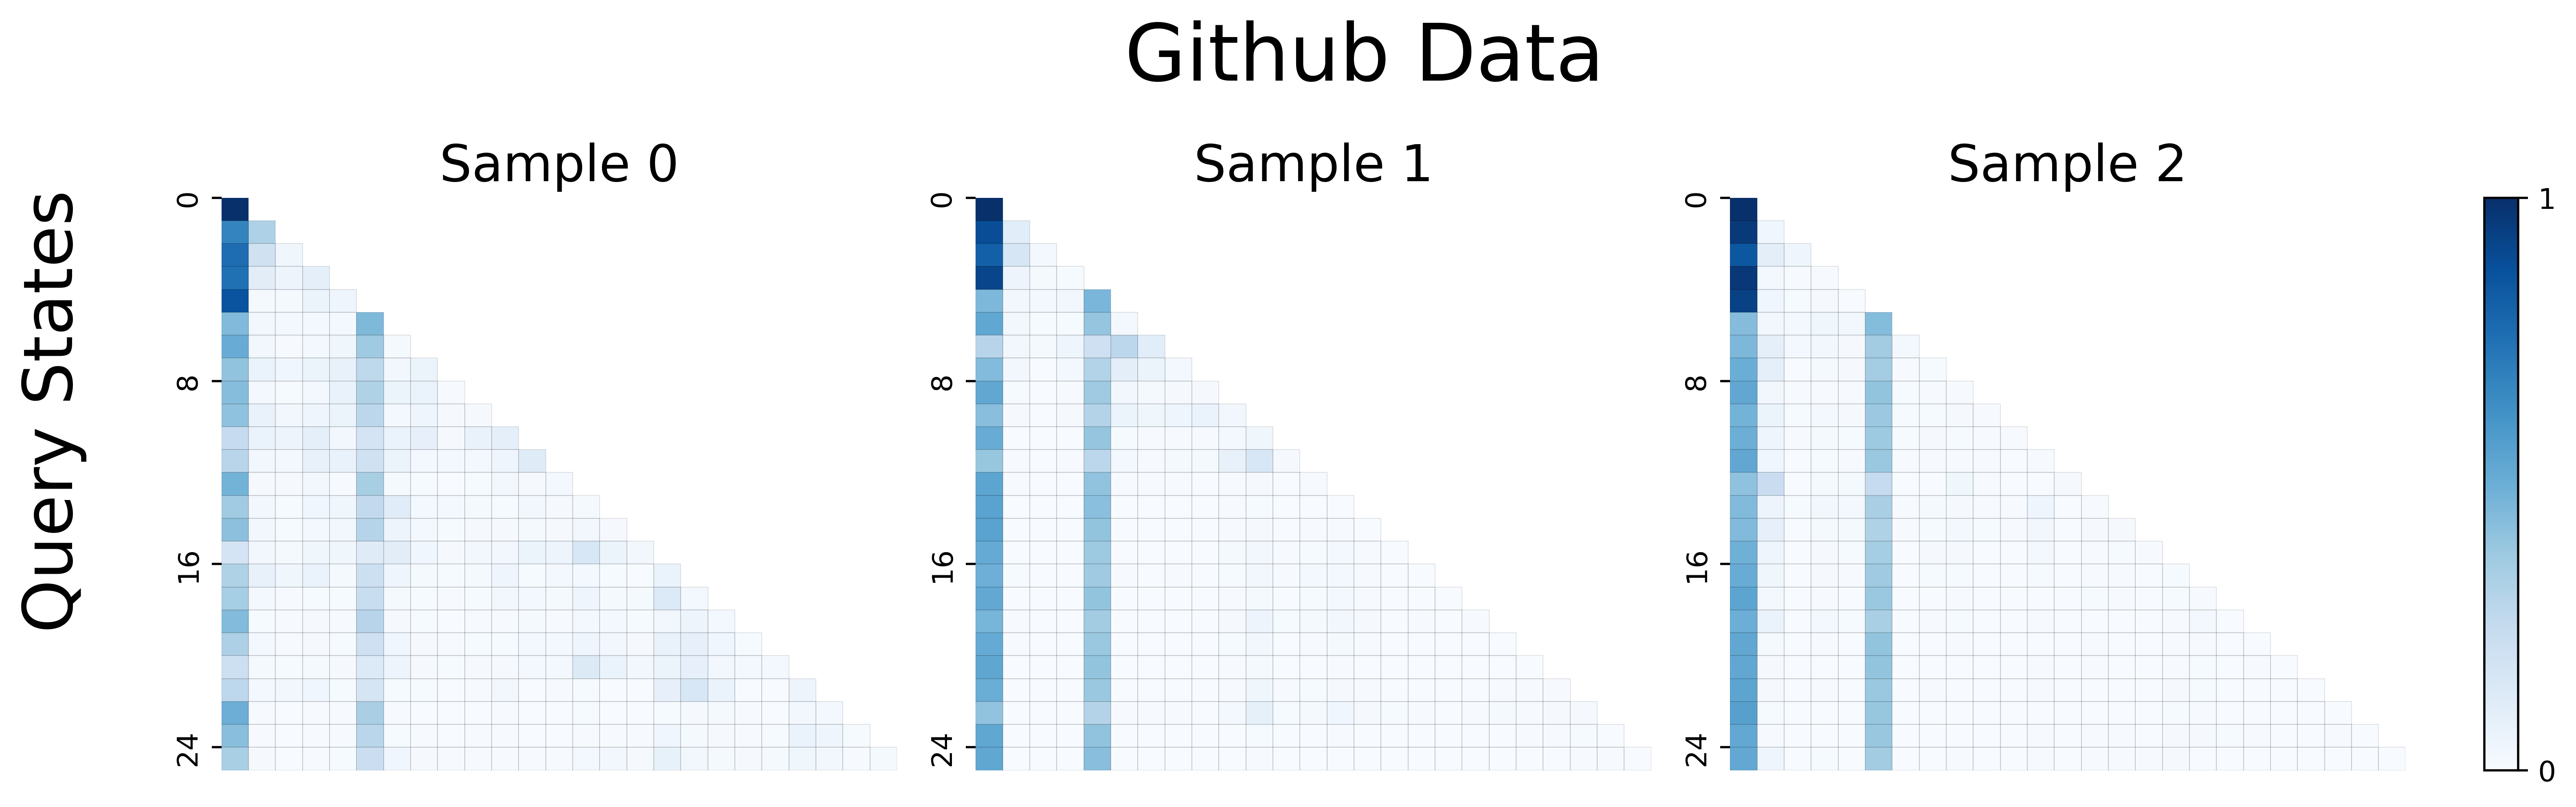
\includegraphics[width=\linewidth]{Figures/L16H20/attn_github_head20.png}
        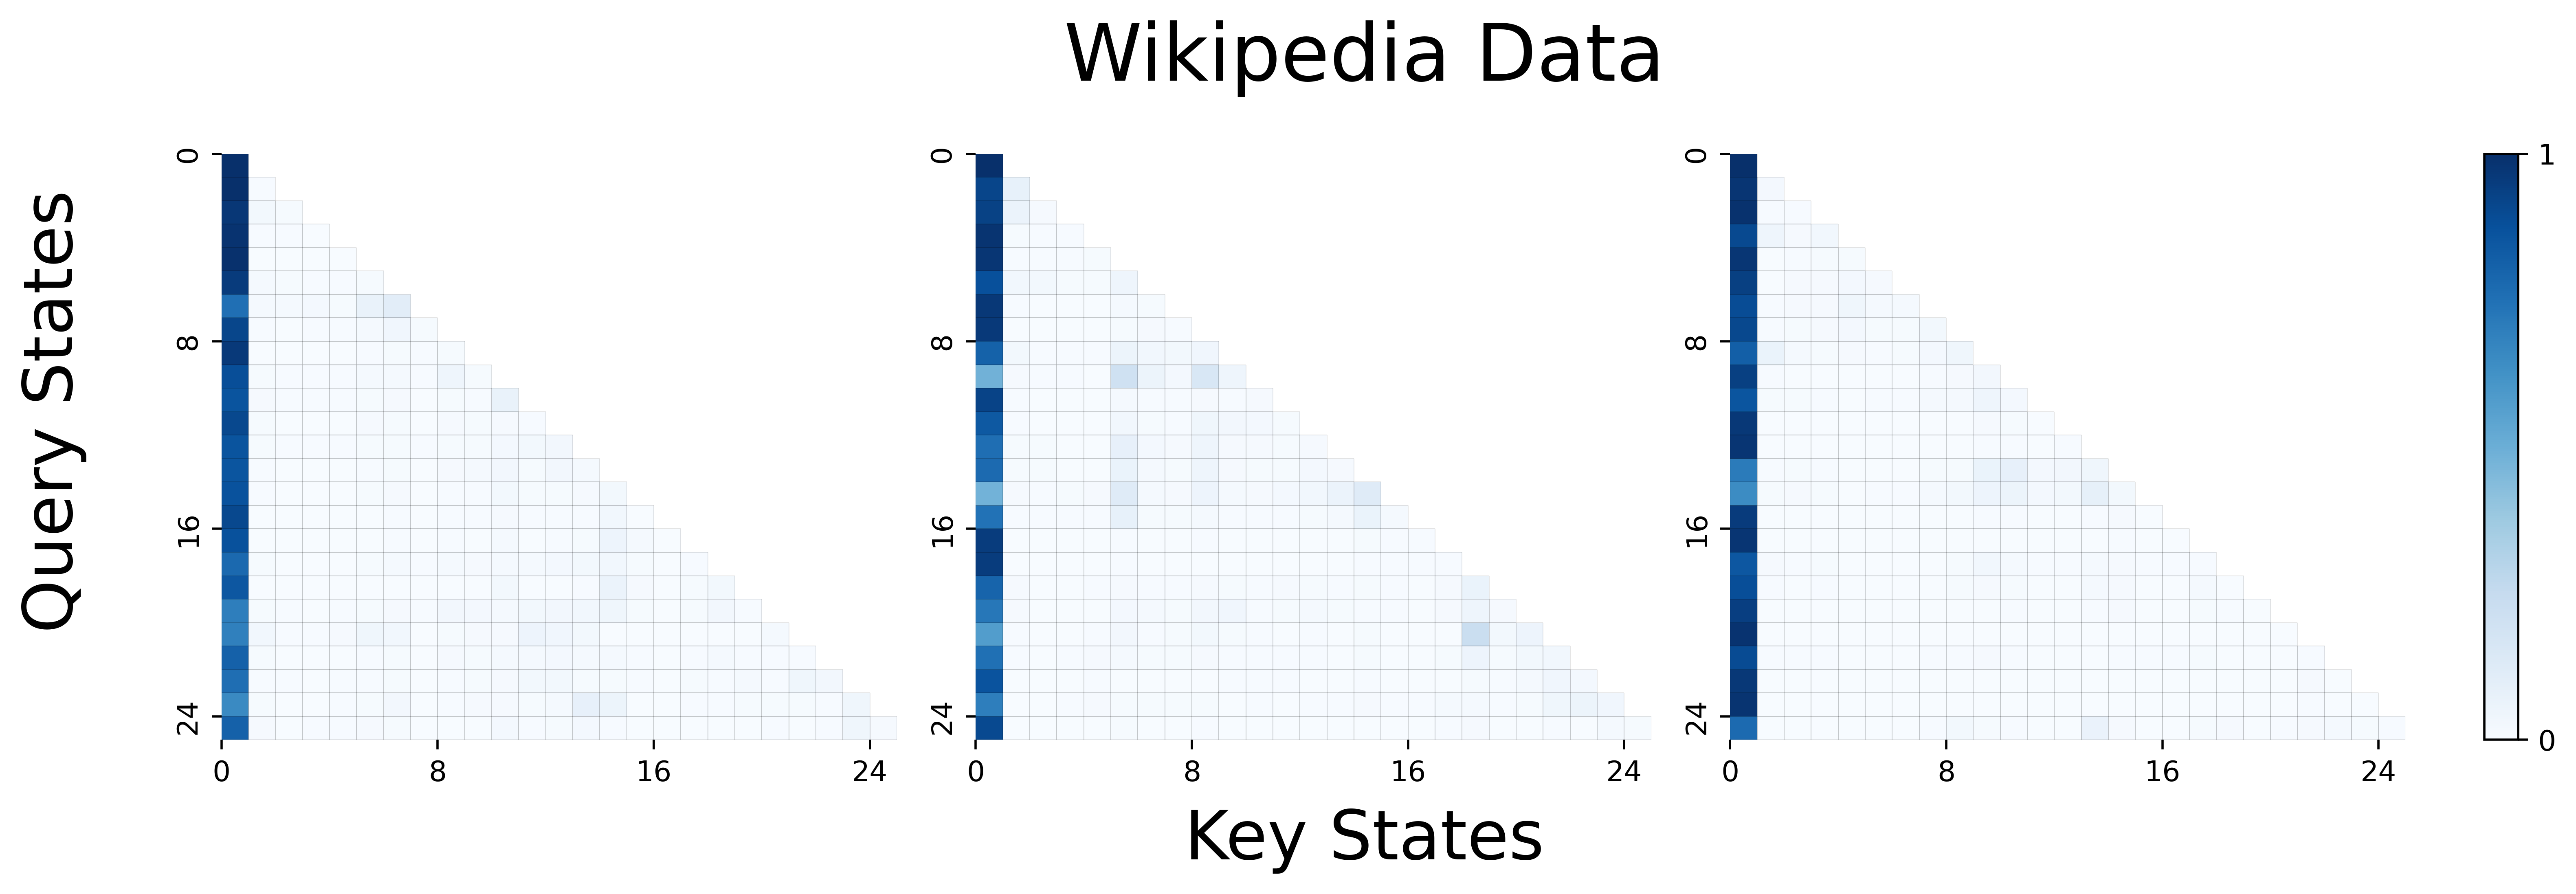
\includegraphics[width=\linewidth]{Figures/L16H20/attn_wikipedia_head20.png}
    \end{subfigure}
    \hfill
    \begin{subfigure}{0.4\textwidth}
        \centering
        \caption{Interventions}
        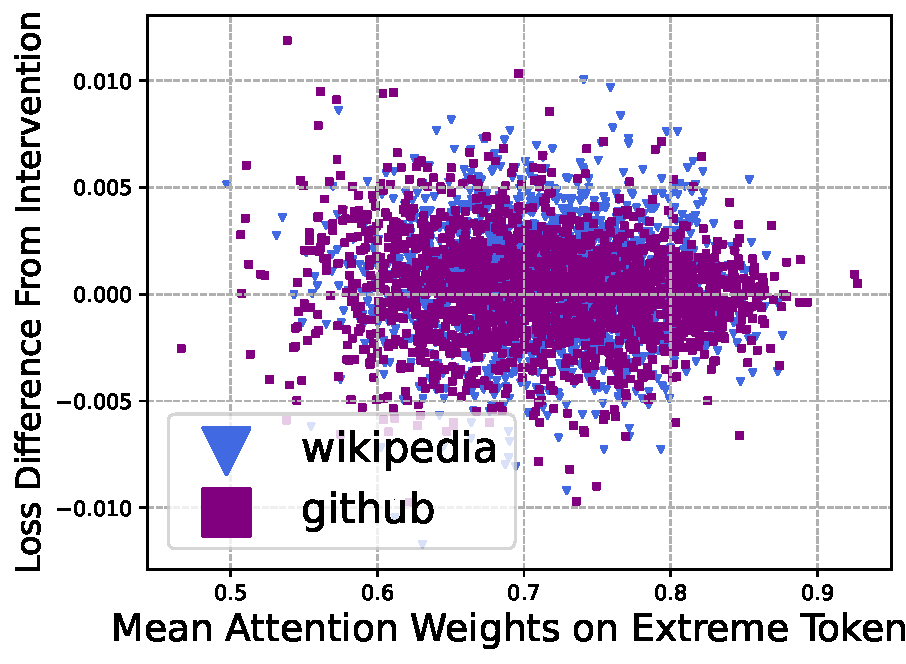
\includegraphics[width=\linewidth]{Figures/L16H20/L16H20.pdf}
    \end{subfigure}
    \caption{\small \textbf{Layer 16 Head 20 of Llama 2-7B-Base.} We do not observe difference between the Wikipedia data and the Github data.}
    \label{fig:llama_l16h20}
\end{figure}

\begin{figure}[h]
    \centering
    \begin{subfigure}{0.575\textwidth}
        \centering
        \caption{Attention patterns}
        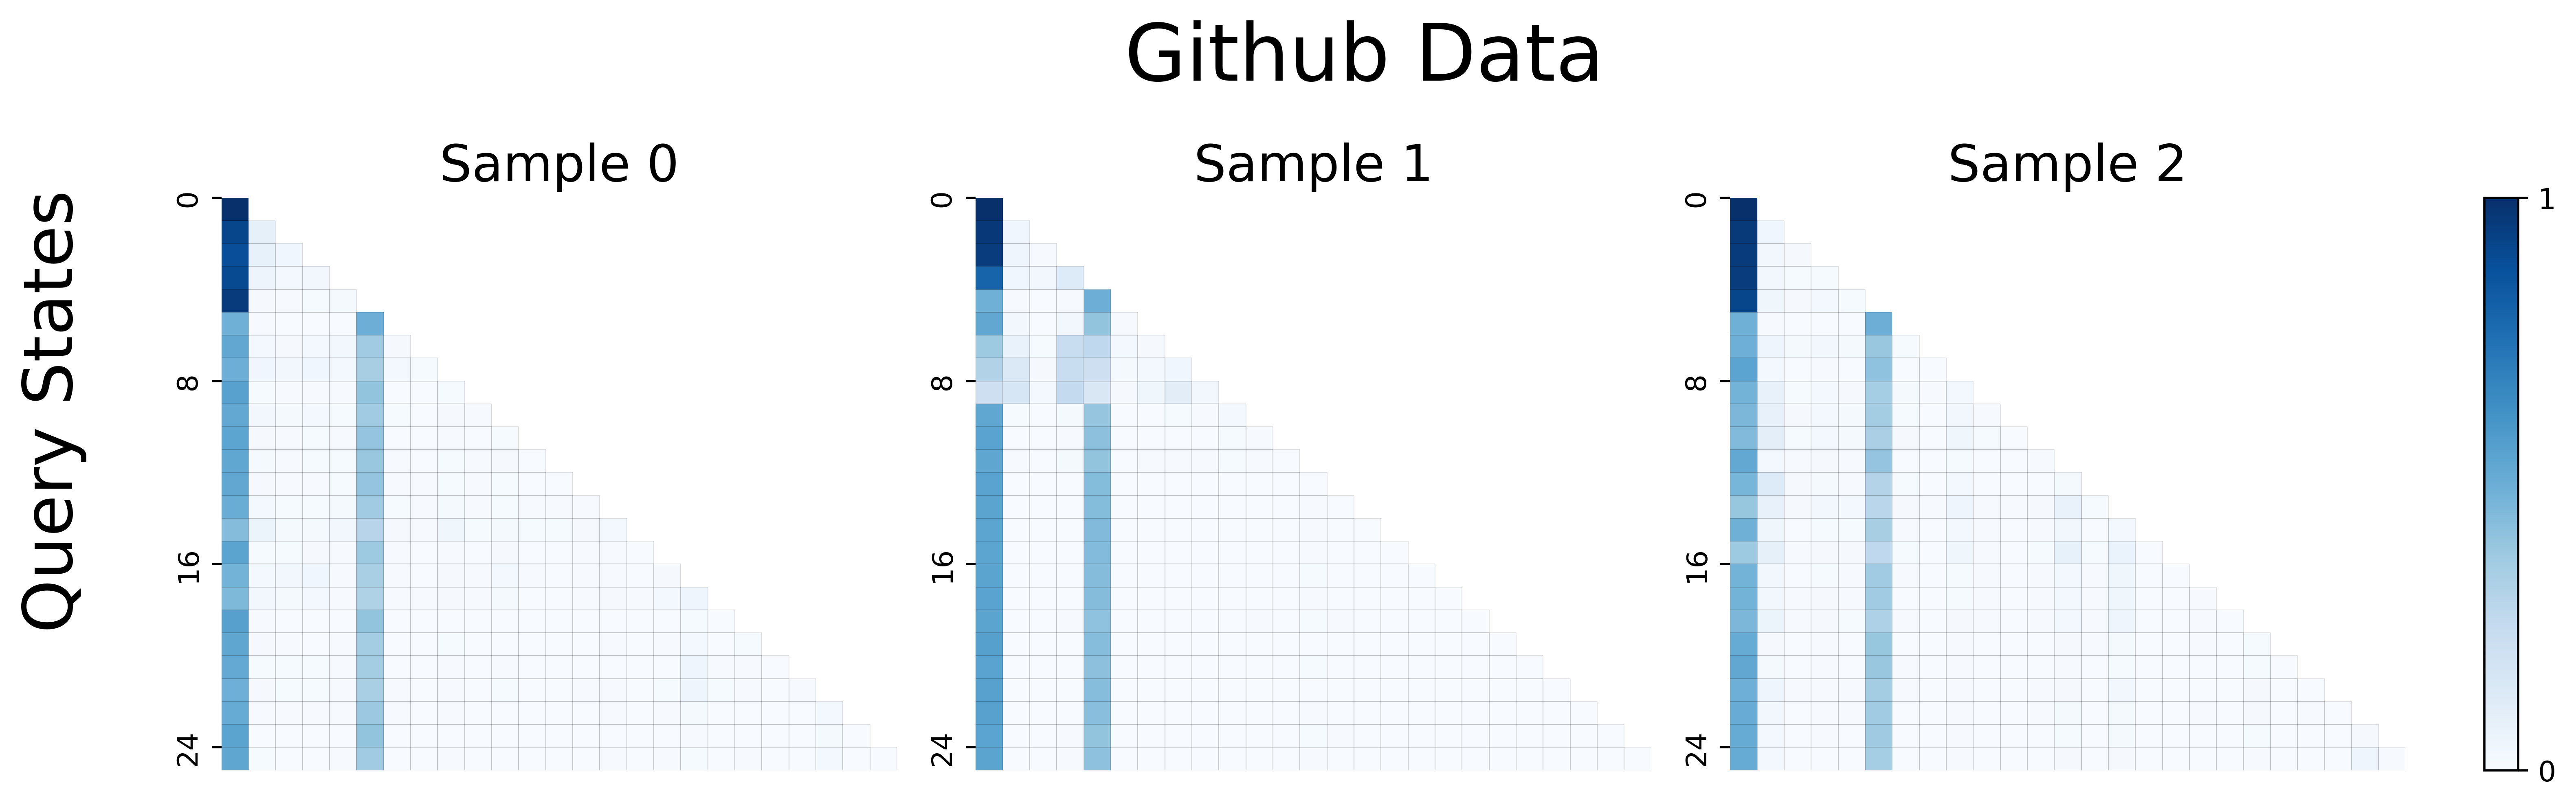
\includegraphics[width=\linewidth]{Figures/L16H28/attn_github_head28.png}
        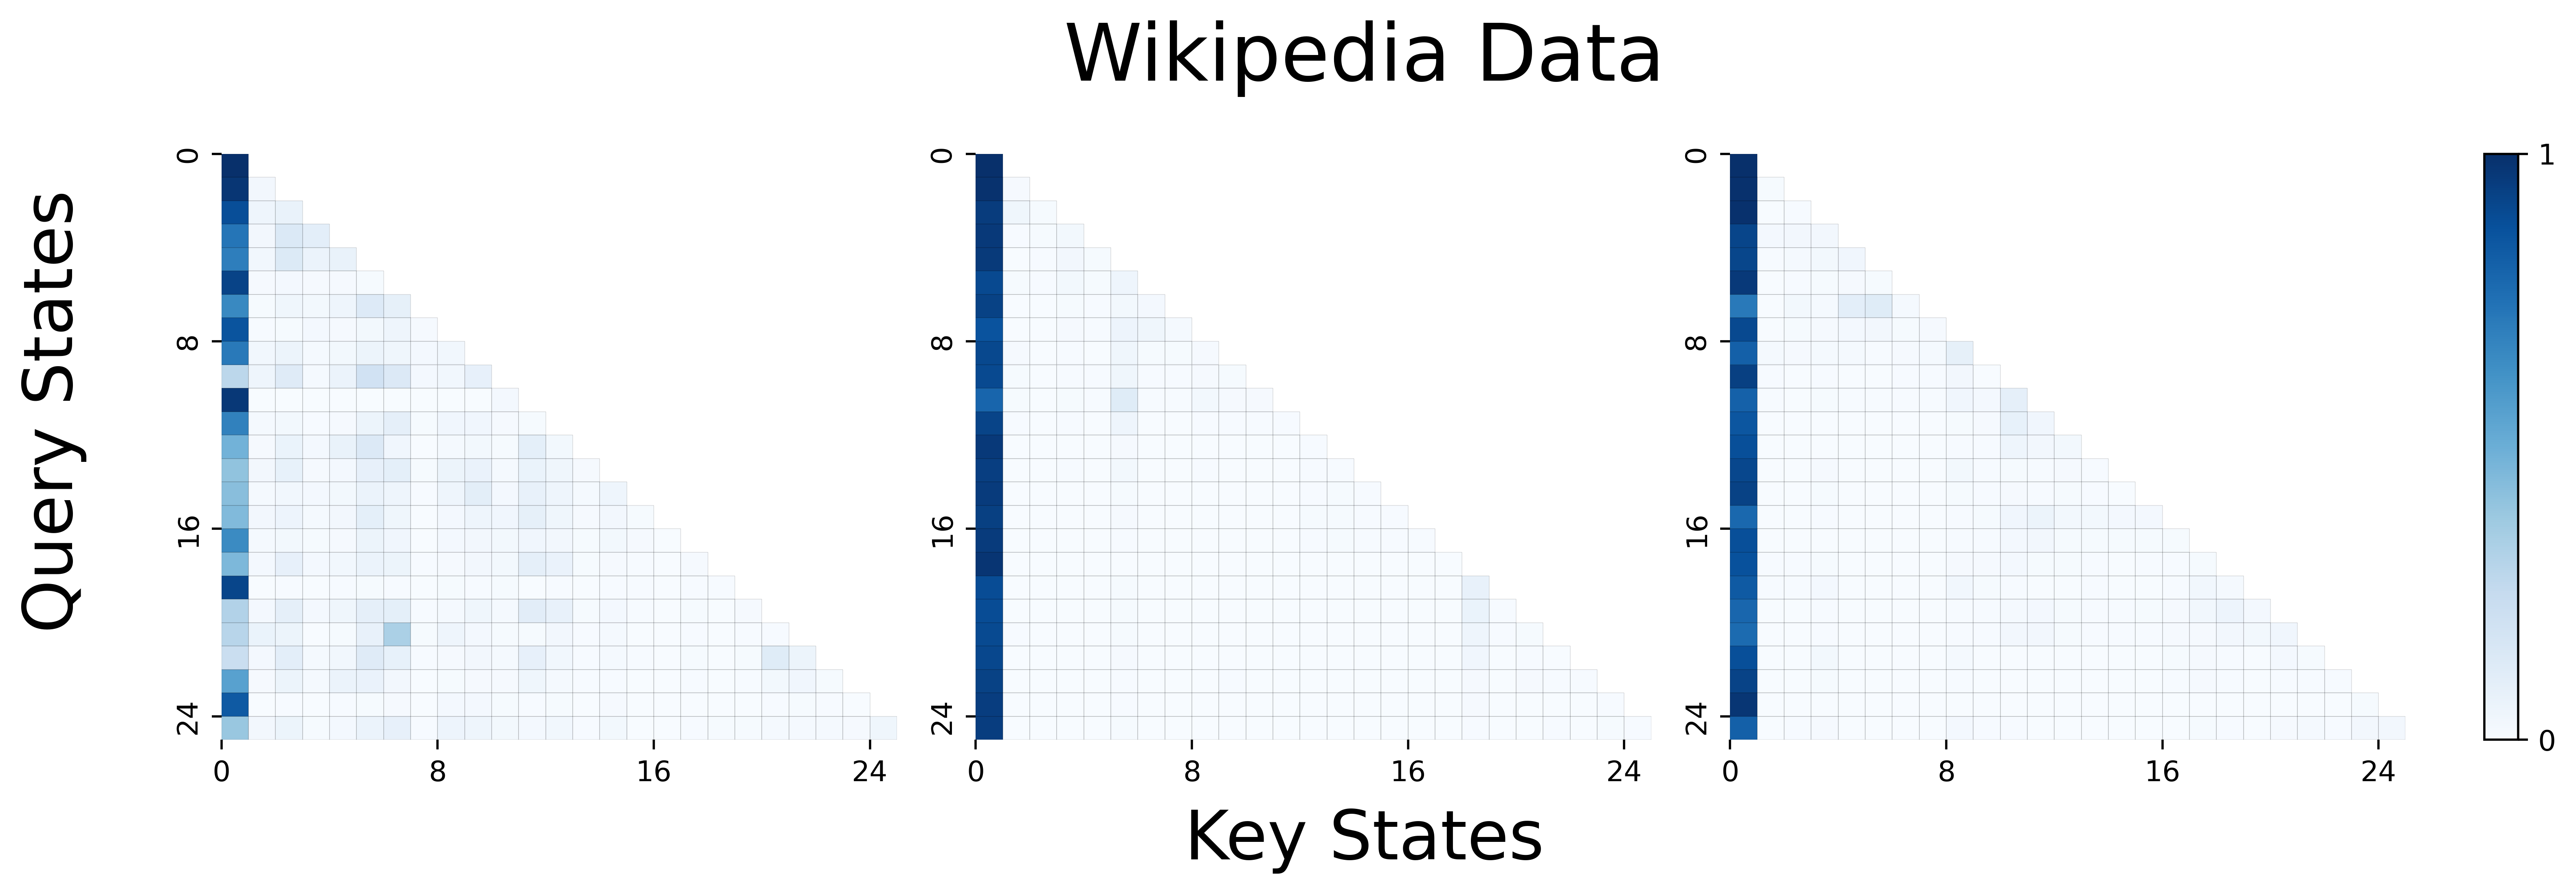
\includegraphics[width=\linewidth]{Figures/L16H28/attn_wikipedia_head28.png}
    \end{subfigure}
    \begin{subfigure}{0.4\textwidth}
        \centering
        \caption{Interventions}
        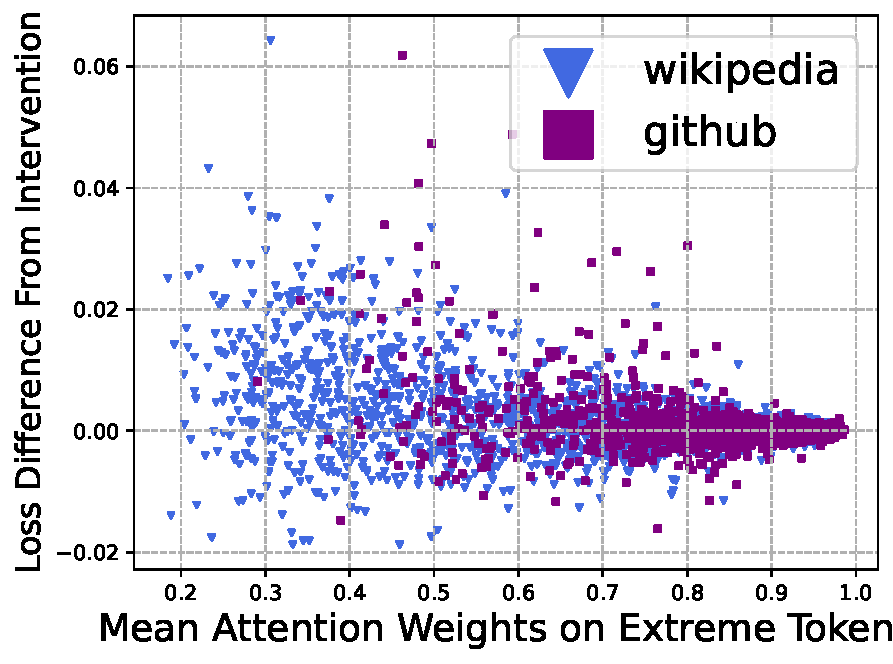
\includegraphics[width=\linewidth]{Figures/L16H28/L16H28.pdf}
    \end{subfigure}
    \caption{\small \textbf{Layer 16 Head 28 of Llama 2-7B-Base.} The head is more dormant on the GitHub data, and more active on the Wikipedia data.}
    \label{fig:llama_l16h28}
\end{figure}


